% "{'chapitre':'dyn_1d','classe':('PSI'),'type':('application'),'titre':'Axe numérique', 'source':'X. Pessoles','comp':[],'corrige':False}"
%\setchapterimage{fig_00}
\chapter*{Application \arabic{cptApplication} \\ 
Axe numérique -- \ifprof Corrigé \else Sujet \fi}

\addcontentsline{toc}{section}{Application \arabic{cptApplication} : Axe numérique -- \ifprof Corrigé \else Sujet \fi}

\iflivret \stepcounter{cptApplication} \else
\ifprof  \stepcounter{cptApplication} \else \fi
\fi
\setcounter{question}{0}

\marginnote{}
\marginnote{
%\UPSTIcompetence[2]{C1-05}
}





Pour aller rechercher des produits dans leurs rayons, Amazon utilise des axes linéaires afin de déplacer un préhenseur.
\begin{marginfigure}
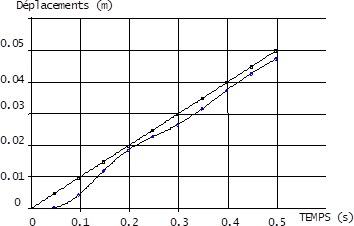
\includegraphics[width=\linewidth]{fig_11}
\end{marginfigure}

Les performances dynamique de l'axe demandées sont les suivantes : 
\begin{itemize}
\item vitesse linéaire maximale : $50 \; \text{m}\,\text{min}^{-1}$;
\item accélération linéaire maximale : $9,8 \; \text{m}\, \text{s}^{-2}$.
\end{itemize}

La loi de commande suivie par l'axe est un trapèze de vitesse. Dans le cas d'un système à un seul axe, l'accélération maximale est toujours atteinte, la vitesse maximale, non.

\begin{obj}
L'objectif de ce travail est de déterminer les caractéristiques du moteur (vitesse et couple) permettant d'atteindre ces performances.
\end{obj}

\question{Quelle est la vitesse maximale que l'axe peut atteindre en  $\text{m}\, \text{s}^{-1}$.}
\ifprof
\begin{corrige}
$V = 0,83 \, \text{ms}^{-1}$
\end{corrige}
\else
\fi

\question{Combien de temps l'axe met-il pour atteindre la vitesse maximale ?}
\ifprof
\begin{corrige}
$T_a =0,83/9,8 = 0,08 s$
\end{corrige}
\else
\fi

\question{Quelle distance l'axe parcourt-il pour atteindre la vitesse maximale ?}
\ifprof
\begin{corrige}
\end{corrige}
\else
\fi


\question{Quelle est la longueur minimale à commander pour que l'axe puisse atteindre la vitesse maximale ?}
\ifprof
\begin{corrige}
\end{corrige}
\else
\fi

\question{Donner les profils de position, vitesse et accélération pour réaliser \SI{5}{cm}.}
\ifprof
\begin{corrige}
\end{corrige}
\else
\fi

\question{Tracer le profil de la position, de la vitesse et de l'accélération pour parcourir une distance de 50 cm. On cherchera à atteindre les performances maximales de l'axe. }
\ifprof
\begin{corrige}
\end{corrige}
\else
\fi


Un motoréducteur permet d'entraîner un système poulie -- courroie permettant de déplacer la charge. On considère :
\begin{itemize}
\item une charge de masse $1\; \text{kg}$;
\item un poulie de rayon $5\; \text{cm}$;
\item un réducteur de rapport de transmission $1:20$.
\end{itemize}

\begin{marginfigure}
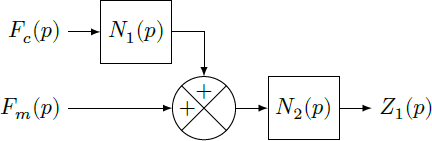
\includegraphics[width=.9\linewidth]{fig_12}
\end{marginfigure}

\question{Déterminer le couple à fournir par la poulie pour déplacer la charge lorsque l'accélération est au maximum. }
\ifprof
\begin{corrige}
\end{corrige}
\else
\fi

\question{Déterminer la vitesse et le couple à fournir par le moteur en considérant que l'inertie du motoréducteur est négligeable. }
\ifprof
\begin{corrige}
\end{corrige}
\else
\fi

\question{Donner la méthode permettant de prendre en compte l'inertie $J$ du motoréducteur ? Quel serait l'impact de la prise en compte de cette hypothèse ? }
\ifprof
\begin{corrige}
\end{corrige}
\else
\fi


\ifprof
\else
\begin{marginfigure}
\centering

\includegraphics[width=3cm]{Cy_01_Ch_03_Application_03_AxeNumerique_qr}
\end{marginfigure}
\fi
